\chapter{Forward Kinematics}

To model the movements of the end effector of a kinematic chain, a forward kinematic analysis is needed. This means, that the position of the endpoint in the operational space needs to be described by the kinematic equations with the joint space as input. The non-linear kinematic equations map the joint parameters to the configuration of the robot system.   This results in a pure geometrical description of motion  by means of position, orientation, and their time derivatives.

\section{Approach}
A serial-link manipulator consists of links in a chain connected by joints. 
A link is a rigid body, defining the spatial relationship between two following axes.
For describing the serial-link mechanism geometry the Denavit Hartenberg notation is one possible approach.
It gives a description of a manipulator for kinematic solutions, Jacobians, dynamics, motion planning and simulation. 
This description can be obtained through a five step algorithm:\cite{ConstantinForwardKA}

\section{Numbering the joints and links}
A serial link robot with n joints has $n+1$ links. 

\paragraph{numbering of links}
The numbering scheme for links starts at $(0)$ with the fixed grounded base and then increases sequentially up to $(n)$ for the end effector.

\paragraph{numbering of joints}
The numbering scheme for joints starts at $(1)$ with the joint connecting the first movable link to the base and then increases sequentially up to n.

\paragraph{relation between links and joints}
Link $(i)$ is connected to its 
\begin{itemize}
	\item lower link $(i-1)$ at its proximal \cite{proxdist} end by joint $(i)$
	\item upper link $(i+1)$ at its distal \cite{proxdist} end by joint $(i+1)$
\end{itemize}

\paragraph{Joint and link numbering in Fanuc 210F}

This numbering scheme can be applied to the Fanuc 210F (see \ref{fig:LinksANDJoints210F}) 


\begin{figure}[H]
	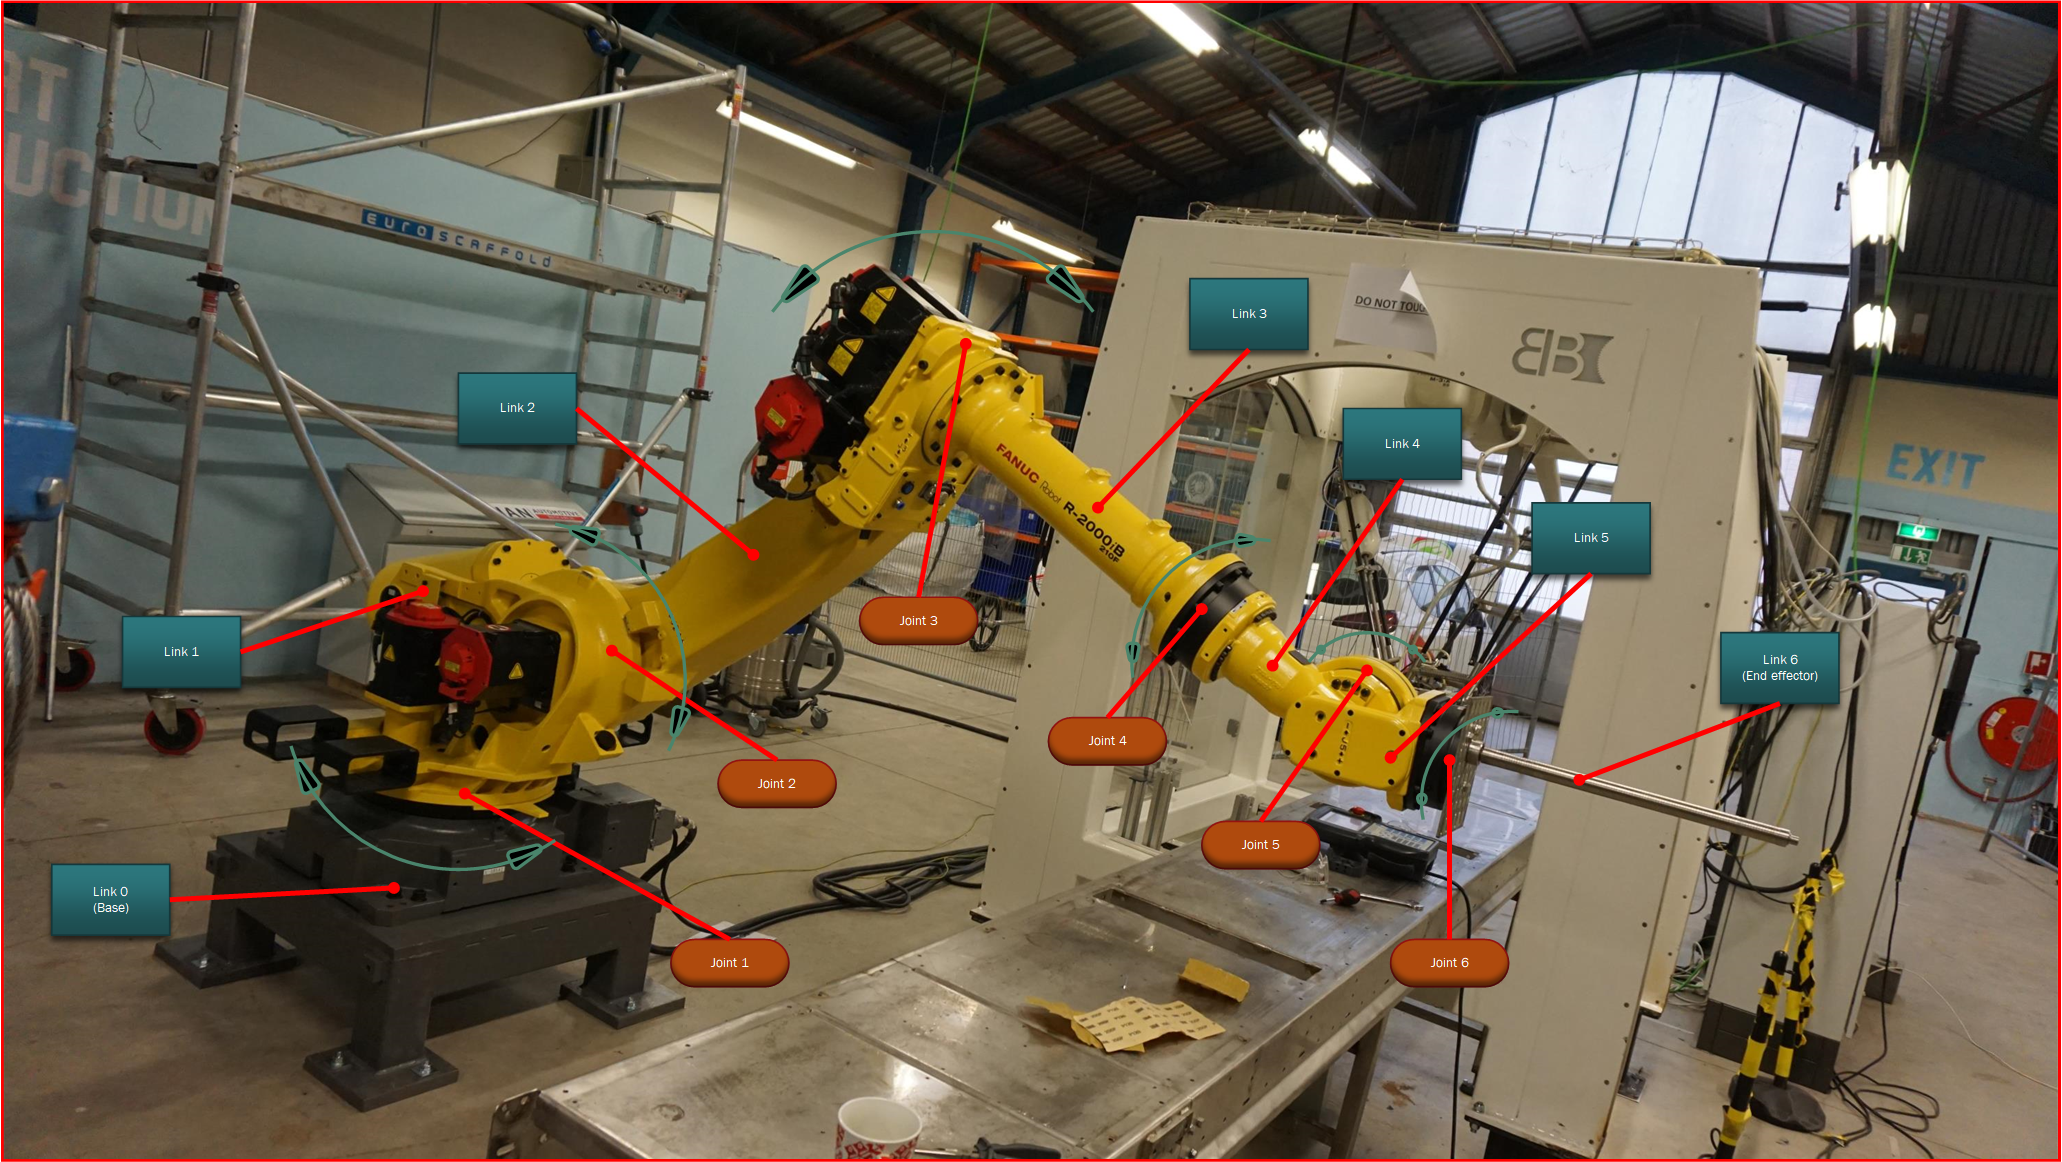
\includegraphics[
	width=1\linewidth,
	center,
	keepaspectratio,
	]{linksANDjoints/linksAndJoints}
	\caption{Links (turquoise) and joints (orange) in the FANUC 210F}
	\label{fig:LinksANDJoints210F}
\end{figure}



\section{local coordinate reference frames}
With the Denavit-Hartenberg convention, local coordinate frames can be attached to the far end of the links $ (i) $ and their accompanying joints $ (i+1) $.
Each link $(i)$ is described relative to the pose of the preceding link.

%\paragraph{Assignation of coordinate frames}


\paragraph{Assignation of $z_i$ axes}

With the DH-notation, the $z_i$ axes are assigned to link $(i)$.
Two cases need to be considered: %regarding joint $(i+1)$:
\begin{itemize}
	\item[revolute:] $z_i$ is the axis of revolution of joint $(i+1)$
	\item[prismatic:] $z_i$ is the axis of translation of joint $(i+1)$
\end{itemize}
%of joint $(i+1)$
This means, that joint $z_i$ turns around axis $z_i$.

\paragraph{Direction of rotation}
With the direction of the $z_i$-axis, the direction of positive rotation around joint $(i+1)$ is also given by the right hand rule (see \cite{Angela_U1S2P1} at 10:35). This means, the direction of positive rotation is counter-clockwise around the $z_i$-axis.

\paragraph{$z_i$ axes in Fanuc 210F}
As described above, the $z_i$ axes can be attached to the Fanuc 210F (see figure \ref{fig:zi_Axes}).

\begin{figure}[H]
	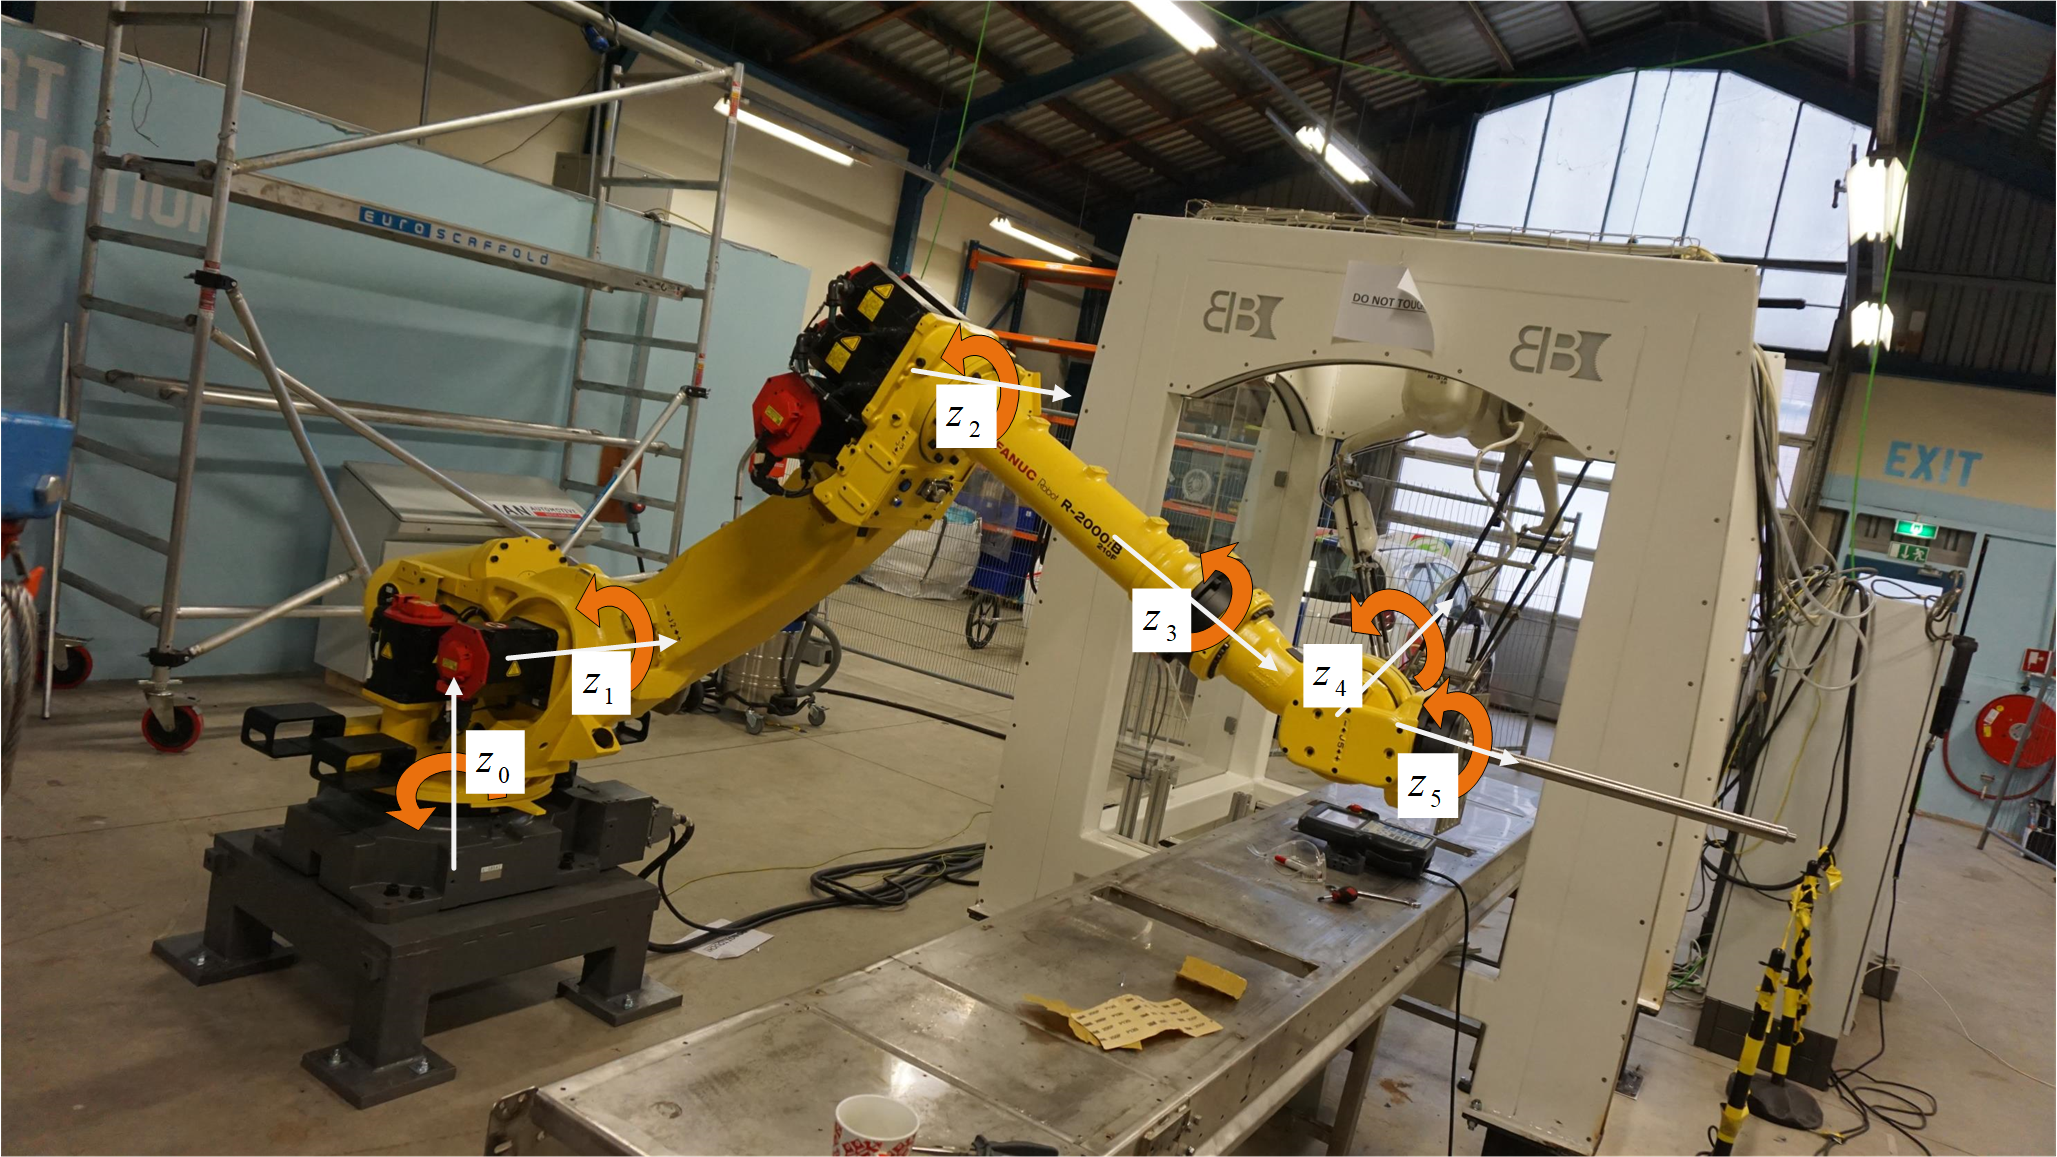
\includegraphics[
	width=1\linewidth,
	center,
	keepaspectratio,
	]{coordinateFrames/z_axes}
	\caption{$z_i$ axes on the Fanuc 210F}
	\label{fig:zi_Axes}
\end{figure}

\paragraph{Base frame}

The base frame $(0)$ can be chosen nearly arbitrarily. Usually, the x-axis of the base frame is chosen, so that it points in the direction of the \ac{EOAT} in default position.

